\newpage
\section{Theoretical Analysis}
\label{sec:analysis}

In this section we will discuss the theoretical analysis of our circuit. For this purpose, we will first explain seperately the Gain stage and the output stage circuits on the Audio Amplifier circuit. The values used throughout this analysis are shown below. 

$V_{ON}$ value is computed using \textit{Ngspice} results for $V_{out}$. By definition, $V_{ON}=\frac{V_{out}}{N_{diodes}}$
\begin{table}[h]
    \centering
    \begin{tabular}{|l|c|}
    \hline
    {\bf Symbol} & {\bf Value} \\ \hline
    $R_{S}$ & $100\Omega$ \\ \hline
    $A_f$ & $12 V$ \\ \hline
    $Audio IN Max$ & $10 mV$  \\ \hline
    $Speaker$ & $8 \Omega$\\ \hline
    \end{tabular}
    \caption{Values for theoretical analysis}
    \label{tab:values}
\end{table}


\subsection{Gain Stage}
\label{sec:gain}

\begin{figure}[!ht] \centering
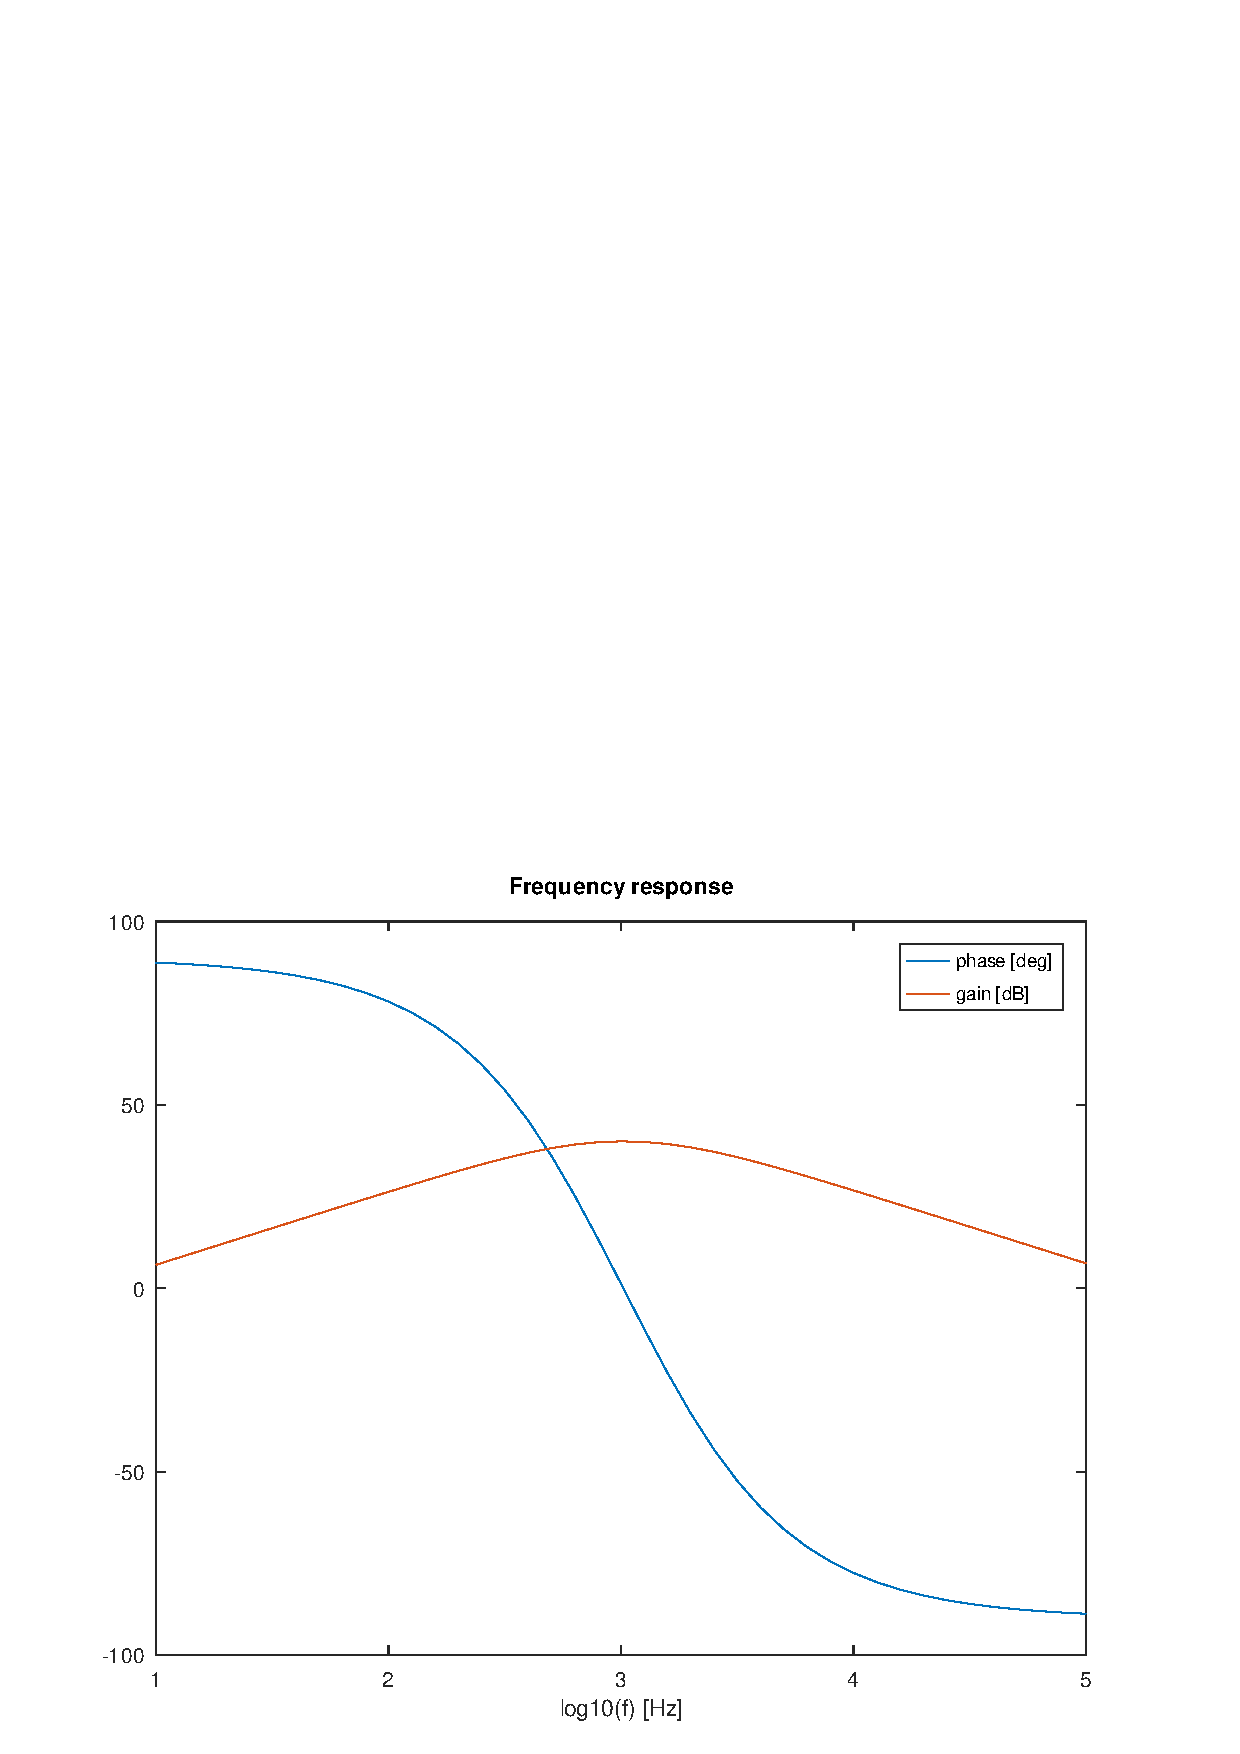
\includegraphics[width=0.8\linewidth]{gain.pdf} 
\squeezeup 
\caption{Gain Stage Circuit.}
\label{fig:gain}
\end{figure}

As seen in figure \ref{fig:gain}...

\subsection{Output Stage}
\label{sec:output}

\begin{figure}[!ht] \centering
    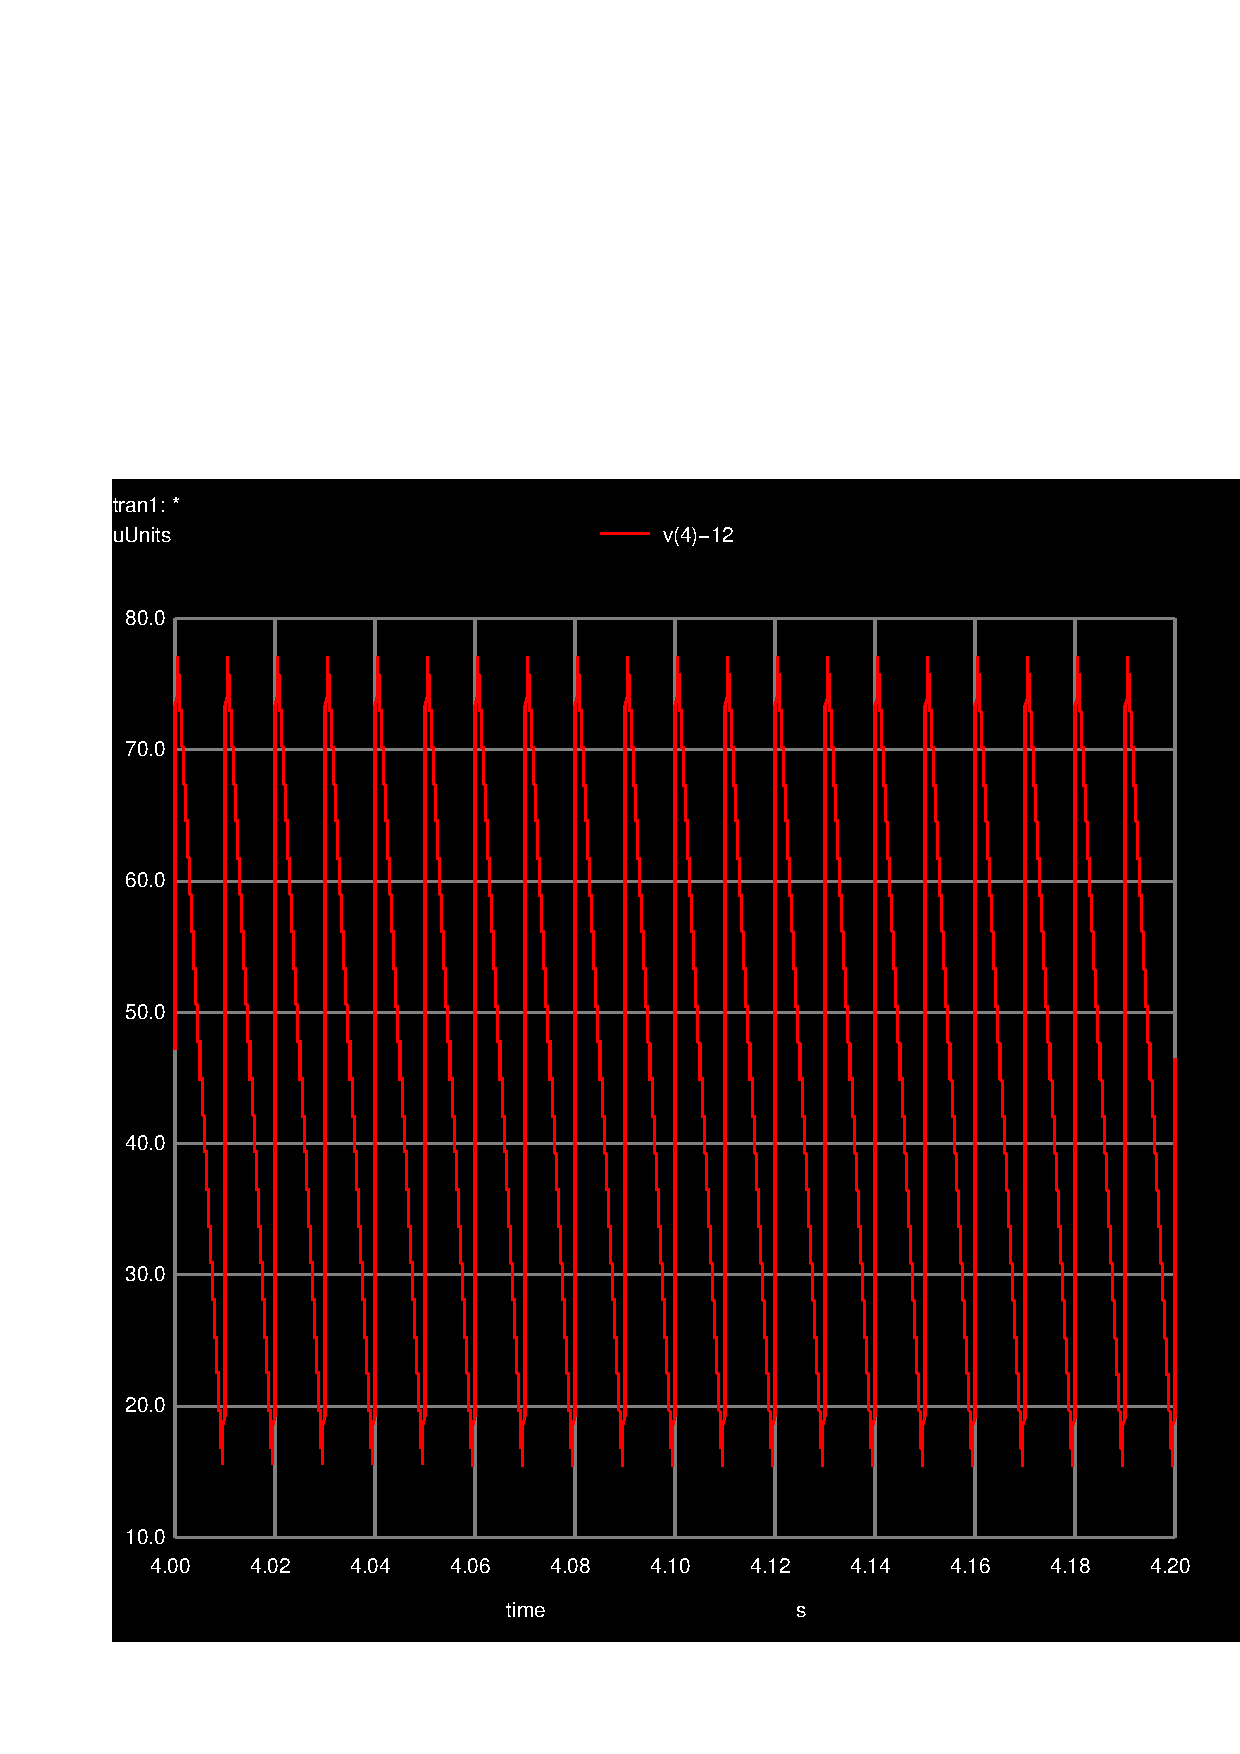
\includegraphics[width=1\linewidth]{output.pdf}
    \caption{Output Stage Circuit.}
    \label{fig:output}
\end{figure}
\newpage




